\documentclass[9pt,a4paper,twocolumn,twoside]{tau-class/tau}
\usepackage[utf8]{inputenc}
\usepackage[slovene]{babel}
\usepackage{amsmath}
\usepackage{graphicx}
\usepackage{booktabs}
\usepackage{listings}

% Komanda za vrednost z aboslutno napako
\newcommand{\abserr}[5]{
    \ensuremath{#1_{#2} = (#3 \ \pm \ #4) \ #5}
}

\newcommand{\relerr}[5]{
    \ensuremath{#1_{#2} = #3 \ (1 \pm \ #4) \ #5}
}

\newcommand{\relativna}[3]{
    \ensuremath{#1 \ (1 \pm #2) \ #3}
}

\newcommand{\absolutna}[3]{
    \ensuremath{(#1 \ \pm \ #2) \ #3}
}


%----------------------------------------------------------
% TITLE
%----------------------------------------------------------

\journalname{Fizikalni eksperimetni III}
\title{Optična rotacija raztopine saharoze}

%----------------------------------------------------------
% AUTHORS, AFFILIATIONS AND PROFESSOR
%----------------------------------------------------------

\author[a]{Matija Zanjkovič}
\affil[a]{Univerza v Mariboru, Fakulteta za naravoslovje in matematiko}


%----------------------------------------------------------
% FOOTER INFORMATION
%----------------------------------------------------------

\institution{Univerza v Mariboru, Fakulteta za naravoslovje in matematiko}
\footinfo{Laboratorijska vaja}
\theday{Junij 2025}
\leadauthor{Zanjkovič Matija}
\author[a]{Mesarec Tilen}
\author[a]{Petauer Maja}
\course{Fizikalni eksperimenti III}

%----------------------------------------------------------
% ABSTRACT AND KEYWORDS
%----------------------------------------------------------

\begin{abstract}
V tej nalogi smo merili optično rotacijo polarizirane svetlobe v raztopinah saharoze različnih koncentracij pri dveh valovnih dolžinah (rdeča in zelena). Iz podatkov smo izračunali specifično rotacijo, ocenili napake in analizirali odvisnost od valovne dolžine z Drudejevo enačbo.
\end{abstract}

\keywords{specifična rotacija, saharoza, Drudejeva enačba, med}

%----------------------------------------------------------

\begin{document}
\setlength{\parindent}{0pt}
        
    \maketitle 
    \thispagestyle{firststyle} 
    \tauabstract 

%----------------------------------------------------------
\section{Uvod}

\taustart{O}ptična rotacija je pojav, kjer kiralne molekule, kot je saharoza, zavrtijo ravnino polarizirane svetlobe. Ta pojav je odvisen od koncentracije snovi $c$, dolžine poti svetlobe $l$ in valovne dolžine $\lambda$. Namen vaje je določiti specifično rotacijo pri različnih koncentracijah in valovnih dolžinah ter preveriti Drudejev model disperzije.

%----------------------------------------------------------
\section{Teorija}

Kot rotacije $\alpha$ je povezan s specifično rotacijo $[\alpha]_\lambda$ preko:
\[
\alpha(\lambda) = [\alpha]_\lambda \cdot c \cdot l
\]
Specifična rotacija je funkcija valovne dolžine in jo lahko približamo z Drudejevim modelom:
\[
[\alpha](\lambda) = \frac{k \lambda^2}{\lambda^2 - A^2}
\]
kjer sta $k$ in $A$ parametra, ki ju določimo iz eksperimentalnih podatkov.

%----------------------------------------------------------
\section{Merjene količine}

\begin{itemize}
    \item \textbf{Koncentracija saharoze} $c$ (g/mL)
    \item \textbf{Valovna dolžina} $\lambda$ (nm),
    \item \textbf{Kot rotacije} $\alpha$ (°), 
    \item \textbf{Dolžina cevi} $l$ (dm)
\end{itemize}


%----------------------------------------------------------
\section{Meritve}

% Dolžina cevi
Dolžina cevi:
\[
\abserr{L}{}{11.5}{0.5}{\text{dm}}
\]
\[
\relerr{L}{}{11.5}{0.043}{\text{dm}}
\]

% Volumen raztopine
Volumen raztopine je bil:
\[
\abserr{V}{}{3000}{60}{\text{mL}}
\]
\[
\relerr{V}{}{3000}{0.02}{\text{mL}}
\]

To smo počeli pri konstantni temperaturi $T = 22 \pm 1 \, \text{°C}$, saj 
na specifično rotacijo vpliva tudi temperatura.\\\\

% Masa saharoze
Masa saharoze je bila izmerjena z napako $3\,\text{g}$. Relativna napaka koncentracije:

\begin{table}[H]
\centering
\begin{tabular}{ccc}
\toprule
$c$ [g/mL] & $\sigma c$ \\
\midrule
0.000 & -- \\
0.030 & 0.033 \\
0.050 & 0.020 \\
0.070 & 0.014 \\
0.090 & 0.011 \\
0.100 & 0.010 \\
\bottomrule
\end{tabular}
\caption{Relativna napaka koncentracije raztopine saharoze.}
\end{table}

Pri meritvah smo opazili, da je pleksi steklo na obeh straneh cevi povzročilo dodatno rotacijo svetlobe. Ta učinek smo upoštevali pri izračunu kotov rotacije.
\begin{table}[H]
\centering
\begin{tabular}{cccc}
\toprule
$c$ [g/mL] & $\alpha_r$ [°] & $\alpha_z$ [°] & $\Delta\alpha$ [°] \\
\midrule
0.000 & 75  & 79  & 2 \\
0.030 & 90  & 96  & 2 \\
0.050 & 102 & 110 & 2 \\
0.070 & 115 & 126 & 2 \\
0.090 & 131 & 136 & 2 \\
0.100 & 137 & 141 & 2 \\
\bottomrule
\end{tabular}
\caption{Izmerjeni koti rotacije za rdečo ($\alpha_r$) in zeleno ($\alpha_z$) svetlobo.}
\end{table}

Meritve z odšteto začetno vrednostjo:

\begin{table}[H]
\centering
\begin{tabular}{cccccc}
\toprule
$c$ [g/mL] & $\alpha_r$ [°] & $\alpha_z$ [°]  & $\Delta \alpha$ [°] & $\sigma \alpha_r$ & $\sigma \alpha_z$ \\
\midrule
0.000 & 0  & 0 & 4 &  \\
0.030 & 15 & 17 & 4 & 0,26 & 0,24 \\
0.050 & 27 & 31 & 4 & 0,15 & 0,13 \\
0.070 & 40 & 47 & 4 & 0,10 & 0,09 \\
0.090 & 56 & 57 & 4 & 0,07 & 0,07 \\
0.100 & 62 & 64 & 4 & 0,06 & 0,06 \\
\bottomrule
\end{tabular}
\caption{Koti rotacije z odšteto začetno vrednostjo za rdečo ($\alpha_r$) in zeleno ($\alpha_z$) svetlobo.}
\end{table}


%----------------------------------------------------------
\section{Izračun specifične rotacije}

Specifična rotacija $[\alpha]$ za vsako meritev:
\[
[\alpha] = \frac{\alpha}{c \cdot L}
\]
kjer je $L$ dolžina cevi (npr. $L = 1$ dm).

\subsection{Rezultati za rdečo valovno dolžino}
\begin{align*}
[\alpha]_{c=0.030} &= 43 \ (1 \pm 0.36) \\
[\alpha]_{c=0.050} &= 47 \ (1 \pm 0.23) \\
[\alpha]_{c=0.070} &= 50 \ (1 \pm 0.17) \\
[\alpha]_{c=0.090} &= 54 \ (1 \pm 0.15) \\
[\alpha]_{c=0.100} &= 54 \ (1 \pm 0.14) \\
\end{align*}

\subsection{Rezultati za zeleno valovno dolžino}
\begin{align*}
[\alpha]_{c=0.030} &= 49 \ (1 \pm 0.33) \\
[\alpha]_{c=0.050} &= 54 \ (1 \pm 0.21) \\
[\alpha]_{c=0.070} &= 58 \ (1 \pm 0.16) \\
[\alpha]_{c=0.090} &= 55 \ (1 \pm 0.14) \\
[\alpha]_{c=0.100} &= 56 \ (1 \pm 0.14) \\
\end{align*}

%----------------------------------------------------------
\pagebreak
\section{Analiza: Drudejev model}

Ker smo specifično rotacijo $[\alpha](\lambda)$ merili pri dveh različnih valovnih dolžinah, smo podatkom prilegli Drudejevo enačbo, ki opisuje odvisnost specifične rotacije od valovne dolžine $\lambda$:
\[
[\alpha](\lambda) = \frac{k \lambda^2}{\lambda^2 - A^2}
\]

Parametra $k$ in $A$ smo določili numerično.


\begin{lstlisting}[language=Python, caption=Numerično prileganje Drudejeve enačbe,
literate={š}{{\v{s}}}1 {Š}{{\v{S}}}1 {č}{{\v{c}}}1 {Č}{{\v{C}}}1 {ž}{{\v{z}}}1 {Ž}{{\v{Z}}}1]
spec_rot_r = [43, 47, 50, 54, 54]  # specifična rotacija za rdečo (primer)
spec_rot_z = [49, 54, 58, 55, 56]  # specifična rotacija za zeleno (primer)
rel_errors_r = [0.36, 0.23, 0.17, 0.15, 0.14]
rel_errors_z = [0.33, 0.21, 0.16, 0.14, 0.14]
lambda_vals = [635]*5 + [532]*5 # valovne dolžine v nm
lambda_errs = [1] * len(lambda_vals)  # napaka +-1 nm

import numpy as np
import matplotlib.pyplot as plt
from scipy.optimize import curve_fit

alpha_vals = np.concatenate((spec_rot_r, spec_rot_z))
alpha_errs_r = [val * rel for val, rel in zip(spec_rot_r, rel_errors_r)]
alpha_errs_z = [val * rel for val, rel in zip(spec_rot_z, rel_errors_z)]
alpha_errs = np.concatenate((alpha_errs_r, alpha_errs_z))

def drude(lambda_nm, k, A):
    return (k * lambda_nm**2) / (lambda_nm**2 - A**2)

params, cov = curve_fit(
    drude,
    lambda_vals,
    alpha_vals,
    sigma=alpha_errs,
    absolute_sigma=True,
    p0=(1e4, 200)
)
k_fit, A_fit = params
k_err, A_err = np.sqrt(np.diag(cov))

print("Ujemajoči parametri:")
print(f"  k = {k_fit:.2f} +- {k_err:.2f}")
print(f"  A = {A_fit:.2f} +- {A_err:.2f} nm")

lambda_fit = np.linspace(450, 700, 300)
alpha_fit = drude(lambda_fit, k_fit, A_fit)

plt.figure(figsize=(8, 5))
plt.errorbar(
    lambda_vals,
    alpha_vals,
    xerr=lambda_errs,
    yerr=alpha_errs,
    fmt='o',
    markersize=6,
    markerfacecolor='steelblue',
    markeredgecolor='black',
    ecolor='gray',
    elinewidth=1,
    capsize=4,
    label='Izmerjeni podatki z napako'
)
plt.plot(lambda_fit, alpha_fit, color='cornflowerblue', linewidth=2.2, label='Drudejevo prileganje')
plt.xlabel('Valovna dolžina lambda (nm)')
plt.ylabel('Specifična rotacija [alpha](lambda)')
plt.title('Prileganje podatkov Drudejevi enačbi')
plt.grid(True, linestyle='--', alpha=0.6)
plt.legend()
plt.tight_layout()
plt.show()
\end{lstlisting}


Rezultati prileganja:
\begin{align*}
\abserr{k}{}{43.88}{11.85}{} \\
\relerr{k}{}{43.88}{0.27}{} \\\\
\noindent \abserr{A}{}{242.28}{146.87}{} \\
\relerr{A}{}{242.28}{0.61}{}
\end{align*}

\begin{figure}[H]
    \centering
    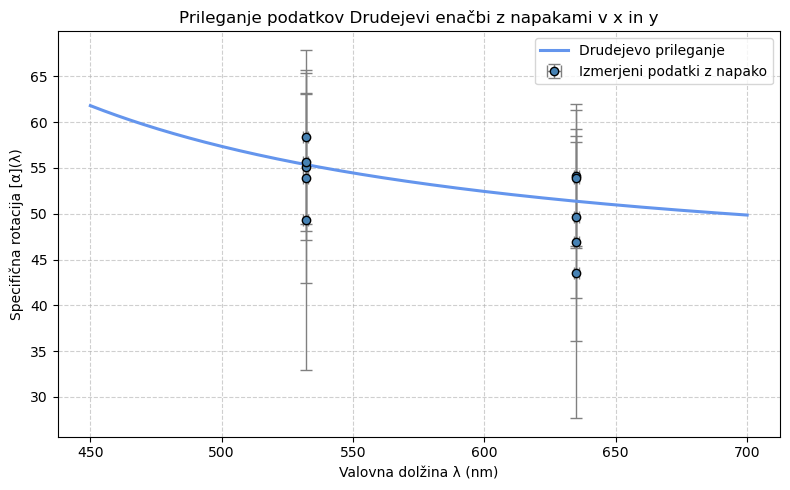
\includegraphics[width=0.9\linewidth]{specrot.png}
    \caption{Prileganje Drudejeve enačbe eksperimentalnim podatkom specifične rotacije.}
    \label{fig:specrot}
\end{figure}

\subsection{Napake in rezultati}

% Rdeči laser (635 nm)
\textbf{Rdeči laser (635 nm):}
\begin{align*}
\abserr{[\alpha]}{635\,\text{nm}}{51}{47}{} \\
\relerr{[\alpha]}{635\,\text{nm}}{51}{0,92}{} \\
\end{align*}

% Zeleni laser (532 nm)
\textbf{Zeleni laser (532 nm):}
\begin{align*}
\abserr{[\alpha]}{532\,\text{nm}}{55}{47}{} \\
\relerr{[\alpha]}{532\,\text{nm}}{55}{0,85}{} \\
\end{align*}

% Modri laser (450 nm)
\textbf{Modri laser (450 nm):}
\begin{align*}
\abserr{[\alpha]}{450\,\text{nm}}{62}{47}{} \\
\relerr{[\alpha]}{450\,\text{nm}}{62}{0,77}{}
\end{align*}

%----------------------------------------------------------
\section{Zaključek}

Eksperiment je pokazal, da se optična rotacija saharoze v vodi spreminja z različnimi koncentracijami in valovnimi dolžinami. Izračunana specifična rotacija potrjuje teorijo o optični aktivnosti in Drudejev model dobro opiše odvisnost od valovne dolžine.

%----------------------------------------------------------
\printbibliography

\end{document}